\documentclass[12pt,a4paper]{article}
\usepackage{enumerate}
\usepackage{fullpage}
\usepackage{amsmath}
\usepackage{graphicx}
\usepackage{verbatim}
\usepackage{parskip}

% Stuff for dot2tex
\usepackage[x11names, rgb]{xcolor}
\usepackage[utf8]{inputenc}
\usepackage{tikz}
\usetikzlibrary{snakes,arrows,shapes}


\title{Stats 391 Project}
\author{By \\ Henry Baba-Weiss, Bill Cauchois, Coral Peterson, and Michael Sloan}
\date{\today}

\begin{document}

\maketitle
\pagebreak

\section { Background }

Tweets are very short messages posted to Twitter, less than 140 characters, that sometimes contain twitter-specific conventions.  The brevity and conventions of Twitter make it a potentially interesting source of information for applying more naive statistical methods / learning techniques.  Many of the Tweets are written to be consumed without other context, making them ideal targets for more simplistic statistical methods.

\section { Description }

The goal of our project is to apply statistical tools to build a model which predicts the ``sentiment'' of tweets.  This ``sentiment'' is dichotomized into just two categories: ``Positive'' and ``Negative''.  The category ``Positive'' is used for posts that would otherwise go into a ``Neutral'' category, if it existed.  By mapping each word in the  is then turned into a vector, and considered to be some indicator that 


\section { Maths }


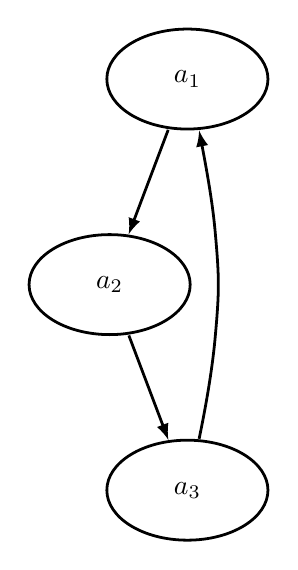
\begin{tikzpicture}[>=latex,line join=bevel,]
  \pgfsetlinewidth{1bp}
%%
\pgfsetcolor{black}
  % Edge: a_2 -> a_3
  \draw [->] (35.921bp,74.708bp) .. controls (39.143bp,66.195bp) and (43.042bp,55.888bp)  .. (50.158bp,37.082bp);
  % Edge: a_3 -> a_1
  \draw [->] (61.215bp,37.471bp) .. controls (63.423bp,48.092bp) and (65.893bp,61.724bp)  .. (67bp,74bp) .. controls (68.517bp,90.821bp) and (68.517bp,95.179bp)  .. (67bp,112bp) .. controls (66.213bp,120.73bp) and (64.737bp,130.14bp)  .. (61.215bp,148.53bp);
  % Edge: a_1 -> a_2
  \draw [->] (50.079bp,148.71bp) .. controls (46.857bp,140.19bp) and (42.958bp,129.89bp)  .. (35.842bp,111.08bp);
  % Node: a_3
\begin{scope}
  \definecolor{strokecol}{rgb}{0.0,0.0,0.0};
  \pgfsetstrokecolor{strokecol}
  \draw (57bp,19bp) ellipse (29bp and 18bp);
  \draw (57bp,19bp) node {$a_3$};
\end{scope}
  % Node: a_2
\begin{scope}
  \definecolor{strokecol}{rgb}{0.0,0.0,0.0};
  \pgfsetstrokecolor{strokecol}
  \draw (29bp,93bp) ellipse (29bp and 18bp);
  \draw (29bp,93bp) node {$a_2$};
\end{scope}
  % Node: a_1
\begin{scope}
  \definecolor{strokecol}{rgb}{0.0,0.0,0.0};
  \pgfsetstrokecolor{strokecol}
  \draw (57bp,167bp) ellipse (29bp and 18bp);
  \draw (57bp,167bp) node {$a_1$};
\end{scope}
%
\end{tikzpicture}



\section{ Implementation }

\subsection { Scraper }

\subsection { Mechanical Turk }

\subsection { Manual Console Categorization }

The console manual categorization program is written in Python, and allows us to respond ``Negative'' or ``Positive'' for a constant stream of posts stored by the scraper.  When the program starts, it looks like this, providing instructions and an initial tweet to categorize:

\begin{verbatim}
enter n for negative, p for positive
vvvvvvvvvvvvvvvvvvvvvvvvvvvvvvvvvvvvvvvvvvvvvvvvvvvvvvvvvvvv
Reality is an illusion that occurs due to lack of alcohol
\end{verbatim}

This is a real tweet encountered while using the tool - one thing we learned from this project is that Twitter users are hilarious and sometime sad.  We were very surprised by the quantity of posts that fell squarely within the ``Negative'' category.  Here's a portion of a contiguous session with the tool:

\begin{verbatim}
____________________________________________________________
vvvvvvvvvvvvvvvvvvvvvvvvvvvvvvvvvvvvvvvvvvvvvvvvvvvvvvvvvvvv
Waiting For The Sun To Go Awayy  So I Could Go Run!
classified as POSITIVE
____________________________________________________________
vvvvvvvvvvvvvvvvvvvvvvvvvvvvvvvvvvvvvvvvvvvvvvvvvvvvvvvvvvvv
I always see people get mad and into argument over the littlest things  and
  I hate arguing .
classified as NEGATIVE
____________________________________________________________
vvvvvvvvvvvvvvvvvvvvvvvvvvvvvvvvvvvvvvvvvvvvvvvvvvvvvvvvvvvv
Finally I have convinced her to abandon her husband  and make our lives one.
classified as NEGATIVE
____________________________________________________________
vvvvvvvvvvvvvvvvvvvvvvvvvvvvvvvvvvvvvvvvvvvvvvvvvvvvvvvvvvvv
he was not sitting on a boar
classified as POSITIVE
____________________________________________________________
vvvvvvvvvvvvvvvvvvvvvvvvvvvvvvvvvvvvvvvvvvvvvvvvvvvvvvvvvvvv
Stressing over history #TheUsual
classified as NEGATIVE
____________________________________________________________
vvvvvvvvvvvvvvvvvvvvvvvvvvvvvvvvvvvvvvvvvvvvvvvvvvvvvvvvvvvv
So James is a whore now? Smh
classified as NEGATIVE
____________________________________________________________
vvvvvvvvvvvvvvvvvvvvvvvvvvvvvvvvvvvvvvvvvvvvvvvvvvvvvvvvvvvv
The most interesting birthday yet... thanks to a very beautiful friend of mine...
  *all smiles*
classified as POSITIVE
\end{verbatim}

It was good to see some extremely positive posts!  Some were also far more ridiculously negative than the examples here.  For more neutral posts, or random posts that likely require more context, the categorization ``Positive'' was used.

\subsection { Manual Web-Based Categorization }



\subsection { Lexer }

One of the main assumptions of this project is that the chosen lexical units, in this case, words, are independent predictors of the classification of the Tweet.  This assumption cannot be correct, for something as complicated as language, but this does imply that the choice of partitioning the lexical units does matter.  Even after we have decided to use single-word lexemes, this leaves us with a few choices:

\begin{enumerate}[1)]
\item How do we handle ``\#hash'' keywords?
\item How do we handle emoticons like ``:)'', ``:('', and ``:')'' - these are the closest thing to a direct encoding of sentiment - so preserving them for the analysis is important!
\item How do we handle ``\&gt;'', ``\&lt;'', and other HTML entities?  These particular examples are interesting, because they are conventionally used to indicate something good (``\&gt;'') or bad (``\&lt;'').
\item How is regular punctuation reported?
\end{enumerate}

Our solution to these considerations was to break the text on the whitespace and punctuation characters.  In order to reasonably handle HTML entities, ``\&'' would be included with any tokens it prefixes, while ``;'' is ignored.  The other punctuation is grouped with adjacent punctuation, and each group reported as a separate word.  This handles the extremely informative punctuation such as emoticons, while also handling regular punctuation.  For example, it can be imagined that ``!'' might oftentimes terminate positive tweets, while ``...'' is used to terminate negative tweets.

\subsection { Bayesian Categorizer }

\subsection { Max-Uncertainty Queue }

One issue with this project is that, similarly to many studies, there is cost associated with taking additional samples.

In the case Mechanical turk, this cost is something on the order of \$0.01 per sample. %TODO: put in real value.

%TODO: consider measuring this better.

In the case of using the manual categorizer, we found that we could categorize tweets at about a rate of about $ 15 \text{tweets} / \text{min} $.  This means that with a solid hour of work, we could categorize 900 tweets.  In order to compute what this means for our price per tweet, we first need an estimate of the value of our time.  If our time is worth the pay of a typical entry-level fulltime software engineer, $ \$40 / \text{hr} $, then each tweet costs $ \$40 \text{min}^{-1} / ( 900 \text{ tweets} * \text{min}^-1 \approx \$0.045 * \text{tweets}^-1 $.  However, we are all in school!  Perhaps it would be more appropriate to use the amount made as a TA: $ \$10.50 * \text{min}^{-1} / ( 900 * \text{tweets} * \text{min}^{-1} ) \approx \$0.015 $.  This is much more in line with the amount that mechanical turk costs.

Either way, it would be cool to make the most of the resource expenditure involved in categorization.  An interesting way of approaching this problem would be to write it down as an optimization problem that relates the cost of data collection with the potential for information gain:

\begin{align*}
\end{align*}



\section { Results }

%TODO: tables, charts, and graphs.

\subsection { Speculation }

%TODO: figure out where to put this / rename.

Tweets use ``hash-tag'' prefixes of words or compounded words in order to indicate some key-word relevant to the contents of your tweet.  In other words, this is a way to even further reduce the amount of content potentially included in your posts, while connecting your post to others'.  


\section { Future Work}

Some ideas for enhancements:

\begin{enumerate}[1)]
\item Use bi-grams / tri-grams.  Instead of just making a distinct choice here, to use, say, bi-grams instead of uni-grams as the unit of association, it would be interesting to 

\item Use more sophisticated models to infer distributions that observe a co-dependency on terms.  In other words, find cases in which the presence of two words in the same tweet is significant, whereas each in isolation is not.

\item Use more sophisticated ways of extracting structure from the individual tweets.  Instead of parsing into tokens that are considered independently, parse into a tree that gives the actual relational structure of the text.  This could then be used to run some sort of trained semantic interpretation of the content.  One way in which this could dramatically affect results is by noticing negations like ``not'', which can entirely invert the sentiment of a Tweet.

\item Use context derivable from the edges derivable from the hash-tag / conversational graph.  This would further inform the previous enhancement idea.
\end{enumerate}

In essence, these further enhancements are each a more sophisticated usage / implementation of NLP (natural language processing) techniques. 

\end{document}